\documentclass[12pt, a4paper]{article}

\usepackage[T1]{fontenc}
\usepackage[utf8]{inputenc}
\usepackage[italian]{babel}
\usepackage{graphicx}
\usepackage{geometry}
\usepackage{xcolor}
\usepackage{enumitem}
\usepackage{setspace}
\usepackage{fancyhdr}
\usepackage{svg}
\usepackage{array}
\usepackage{lastpage}
\usepackage{comment}
\usepackage{caption}
\usepackage{xparse}
\usepackage[colorlinks=true, linkcolor=black]{hyperref}

% Pacchetti necessari per la tabella avanzata
\usepackage{tabularx}
\usepackage{booktabs}
\usepackage{float}

% Pacchetto per risolvere l'errore "Cannot find reference LastPage"
\usepackage{lastpage}

% Correzione per l'avviso di "fancyhdr: \headheight is too small"
\setlength{\headheight}{15pt}

\renewcommand{\contentsname}{Indice}
\renewcommand{\sectionmark}[1]{\markboth{#1}{#1}}

\pagestyle{fancy}
\fancyhf{}
\fancyhead[L]{\nouppercase{\leftmark}}
\fancyhead[R]{pagina \thepage\ di \pageref*{LastPage}}

\geometry{
	top=2.5cm,
	bottom=2.5cm,
	left=3cm,
	right=3cm
}

% Spacing between figure and surrounding text
\setlength{\textfloatsep}{20pt}
\setlength{\intextsep}{20pt}

% Caption style (optional tweaks)
\captionsetup{
	font=small,
	labelfont=bf,
	skip=6pt
}

% Save originals before redefining
\let\origincludegraphics\includegraphics
\let\origincludesvg\includesvg

% Redefine \includegraphics[options]{file}{optional caption}
\RenewDocumentCommand{\includegraphics}{O{width=\linewidth} m g}{%
	\begin{figure}[htbp]
		\centering
		\origincludegraphics[#1]{#2}%
		\IfValueT{#3}{\caption{#3}}%
	\end{figure}%
}

\NewDocumentCommand{\insertsvg}{O{width=\linewidth} m g}{%
	\begin{figure}[htbp]
		\centering
		\let\includegraphics\origincludegraphics% prevent nested figure
		\includesvg[#1, inkscapelatex=false]{#2}%
		\IfValueT{#3}{\caption{#3}}%
	\end{figure}%
}

\definecolor{criticalred}{RGB}{192, 0, 0}

\renewcommand{\abstractname}{Sommario}

\begin{document}

\begin{titlepage}
		\centering
		
		\origincludesvg[width=0.6\textwidth]{assets/logoUnisa.svg}		
        
		\vspace{4cm}

		{\Huge\bfseries Penetration Testing Report}
		
		\vspace{0.6cm}
		
		{\LARGE\color{gray} Academy -- Cybersecurity}
		
		\vspace{2.5cm}
		
		{\large Kioptrix Level 1}
		
		\vspace{1.6cm}
		
		{\Large\bfseries Gruppo 15}
		
		\vspace{0.6cm}
		
		\begin{tabular}{>{\raggedleft\arraybackslash}p{6cm}@{\;--\;}p{6cm}}
			0612709539 & Francesco Cangianiello \\
			0612709671 & Andrea Ciliberti \\
			0612709638 & Serena Fierro \\
		\end{tabular}
		
		\vfill
		
		{\small A.A. 2025/2026}
		
	\end{titlepage}

	\newpage 

	\begin{abstract}
		Il presente documento costituisce il report dell'attività di \textbf{Penetration Testing} condotta sulla macchina identificata come "Kioptrix Level 1". 
		
		L'obiettivo è stato valutare la sicurezza del sistema attraverso la simulazione di un attacco informatico mirato, eseguito secondo una metodologia \textbf{BlackBox} (senza alcuna conoscenza pregressa o credenziale fornita).
		
		L'analisi ha evidenziato un sistema profondamente vulnerabile a causa di una spessa obsolescenza software. Sono state identificate complessivamente \textbf{130 evidenze di insicurezze}, tra cui spiccano \textbf{3 vulnerabilità di livello critico (CVSS 10.0)} a carico dei servizi di rete e del sistema operativo. Lo sfruttamento di tali falle ha permesso di bypassare ogni meccanismo di difesa e di ottenere l'accesso remoto con i massimi privilegi di amministrazione (\textbf{root}), portando alla compromissione totale del sistema.
		
		Lo scopo di questo report è di illustra l'impatto sulla sicurezza, fornire una panoramica chiara dei vettori di attacco testati e mostrare un piano di \textbf{Remediation} per mitigare i rischi e mettere in sicurezza l'asset.
	\end{abstract}

	\newpage
	\thispagestyle{empty}
	\tableofcontents

	\newpage
	\section{EXECUTIVE SUMMARY}
	\subsection{Obiettivo dell'Incarico}
	Nel periodo compreso tra il 26/05 e il 16/06, il nostro team ha condotto un \\ \textbf{Penetration Test} mirato sull'infrastruttura identificata come "Kioptrix Level 1".\\

	\raggedright L'attività è stata progettata per simulare un attacco \textbf{informatico realistico}, con lo scopo di identificare le vulnerabilità presenti nel sistema e verificarne l'impatto attraverso tecniche di sfruttamento (\textbf{exploitation}).\\
	Nello specifico, i test si sono concentrati sulla valutazione del rischio reale, verificando se un attaccante esterno potesse arrivare a ottenere un accesso remoto non autorizzato con i massimi privilegi di amministrazione (\textbf{root}).\newline

	\raggedright L'obiettivo finale di questa simulazione è stato quello di testare la resilienza della macchina ed \textbf{evidenziare le criticità di sicurezza}, 
	fornendo indicazioni chiare per la loro mitigazione prima che queste potessero essere sfruttate attivamente da attori malevoli.
\newline
	
	\subsection{Risultati ottenuti}
	Durante l'analisi automatizzata e manuale dell'infrastruttura sono state rilevate complessivamente \textbf{130 vulnerabilità}.\\
	Tra queste, spiccano \textbf{5 vulnerabilità di livello Critico} e \textbf{18 di livello Alto}, che espongono l'asset analizzato a un rischio grave.\\
	Nel dettaglio:

	\begin{itemize}
		\item \textbf{Compromissione del Perimetro Esterno (Servizio Web):} I servizi esposti al pubblico utilizzano componenti crittografici obsoleti e non più sicuri.
		Sfruttando questa debolezza, un attaccante esterno può eludere completamente le misure di sicurezza e ottenere un accesso remoto non autorizzato alla macchina.\\ 
		Questo scenario apre la strada ad \textbf{attacchi più profondi}, pur in totale assenza di credenziali valide.
		\item \textbf{Difetto Strutturale e Dominio Totale (Sistema Operativo):} La base del sistema operativo (\textbf{Kernel Linux}) ha ampiamente superato il suo ciclo di vita e presenta difetti strutturali impossibili da correggere con semplici aggiornamenti. 
		Sfruttando un accesso iniziale anche limitato (come quello ottenuto violando il servizio web), un attaccante può aggirare le restrizioni di sicurezza e scalare i propri privilegi fino a diventare amministratore della macchina, esponendo la macchina a gravi problemi.
		\newpage
		\item \textbf{Esposizione dei Dati e Controllo Immediato (Condivisione File):} Il sistema che si occupa della condivisione delle risorse di rete (Samba) presenta \textbf{gravi misconfiguration e componenti non aggiornati}.
		Questa esposizione genera un duplice rischio: 
		\begin{itemize}
			\item[*] da un lato, permette a chiunque di interrogare il sistema e raccogliere informazioni aziendali sensibili in forma completamente anonima.
			\item[*] dall'altro, espone il server ad attacchi diretti e automatizzabili che garantiscono all'attaccante l'acquisizione immediata dei massimi privilegi amministrativi, avendo il pieno controllo della macchina.
		\end{itemize} 
		
	\end{itemize}

	\vspace{2 cm}

	\subsection{Valutazione Globale del Rischio}
	Il \textbf{livello di rischio complessivo} per il sistema analizzato è valutato come \textbf{CRITICO}.\\
	L'infrastruttura presenta gravi carenze di sicurezza derivanti dall'utilizzo di servizi di rete (come server web e protocolli di condivisione file) e componenti di base obsoleti e non più supportati. \\
	Tali criticità permettono a un potenziale attaccante esterno, anche senza disporre di alcuna credenziale di accesso, di sfruttare vulnerabilità pubbliche note per eseguire codice arbitrario e ottenere il controllo totale della macchina con i massimi privilegi (root). 
	Questo scenario compromette integralmente la riservatezza, l'integrità e la disponibilità del sistema. \newline

	\newpage
	\subsection{Raccomandazioni Strategiche (Contromisure)}

	Per riportare il livello di rischio entro soglie accettabili e proteggere l'infrastruttura da compromissioni simili, si raccomanda alla Direzione di dare priorità alle seguenti iniziative: 
	\begin{itemize}
		\item \textbf{Revisione dei Controlli di Accesso:} Richiedere al team di sviluppo un intervento immediato per validare correttamente i permessi degli utenti su ogni richiesta applicativa.
		\item \textbf{Gestione degli Aggiornamenti:} Richiede una fase importante di identificazione e installazione tempestiva degli aggiornamenti di sicurezza sui servizi esposti e sul sistema operativo usato.
		\begin{itemize}
			\item[*] Qualora non sia possibile aggiornare componenti datati per ragioni tecniche o di compatibilità, è importante isolare la macchina a livello di rete (come mediante regole firewall rigide) per limitare i danni in caso di compromissione, oppure procedere con la temporanea dismissione del servizio in questione.
 		\end{itemize}
		\item \textbf{Minimizzazione della Superficie di Attacco:} Disabilitare tutte le porte e i servizi di rete non strettamente necessari all'operatività aziendale. Un'attenta configurazione riduce drasticamente i punti di ingresso a disposizione di un potenziale attaccante. 
	\end{itemize}



	\newpage
	\section{ENGAGEMENT HIGHLIGHTS}

	\subsection{Definizione accordi preliminari tra le parti coinvolte}
	L'attività è stata concordata tra il \textbf{cliente} e il \textbf{team di Security Assessment} (Gruppo 15).\\ 
	L'accordo prevede la simulazione di un \textbf{attacco informatico} controllato al fine di mappare lo stato di sicurezza dell'asset, identificare le criticità e fornire le relative misure di mitigazione (Remediation).\\
	\vspace{0.5 cm}
	\textbf{Periodo di esecuzione:} Da Maggio 2026 a Giugno 2026.\\
	\vspace{0.5 cm}
	\textbf{Target:} Macchina virtuale "Kioptrix Level 1".


	\subsection{Requisiti legali e operativi stabiliti prima dell’avvio del test}
	Prima dell'avvio delle scansioni, sono stati definiti e rispettati i seguenti \textbf{vincoli operativi}:
	\begin{itemize}
		\item \textbf{Autorizzazione Formale:} Il team è stato esplicitamente autorizzato a condurre attività di port scanning, vulnerability assessment , tentativi di intrusione (exploitation) e Maintaining Access sul target concordato.
		\item \textbf{Isolamento dell'Ambiente:} Al fine di rispettare i requisiti legali e prevenire qualsiasi interferenza con reti esterne o sistemi di terze parti, i test sono stati eseguiti esclusivamente all'interno di un ambiente di laboratorio chiuso e rigorosamente segmentato (Rete NAT).
	\end{itemize}

	\subsection{Modalità di esecuzione del penetration testing}
	L'attività di attacco e analisi è stata eseguita secondo le seguenti specifiche tecniche:
	\begin{itemize}
		\item \textbf{Approccio: BlackBox (Scansione non Autenticata).} Il team ha operato senza alcuna conoscenza pregressa dell'infrastruttura, dei servizi in esecuzione o delle credenziali di accesso.
		\item \textbf{Ambito di scansione (Port Scan):} È stato configurato il controllo completo su tutte le porte TCP nel range 1-65535.
		\item \textbf{Profondità dei test web:} È stata eseguita sia la scansione automatica dei servizi sia il crawling mirato delle directory applicative con l'obiettivo di ottenere file o configurazioni nascoste.
	\end{itemize}

	\newpage
	\subsection{Metodologia adottata}
	E' stato adottato un approccio strutturato combinando test automatici e verifiche manuali attraverso i seguenti strumenti:
	\begin{itemize}
		\item \textbf{Vulnerability Scanning di Rete}: Utilizzo di \textbf{OpenVAS} (configurazione: Full and Fast) e \textbf{Nessus} (configurazione: Basic Network Scan \& Web Application tests).
		\item \textbf{Vulnerability Scanning Web}: Impiego di \textbf{Nikto} per l'analisi delle vulnerabilità del server Apache e del modulo mod\_ssl.
		\item \textbf{Directory Crawling}: Utilizzo di \textbf{Dirb} e \textbf{Gobuster} per l'esplorazione delle cartelle del server web (scoprendo l'assenza di pagine pubblicate e l'istanza isolata di Webalizer).
	\end{itemize}

	\subsection{Obiettivi del test}
	L'ingaggio si è posto i seguenti obiettivi chiave:
	\begin{itemize}
		\item \textbf{Identificare e catalogare tutte le vulnerabilità} presenti sull'asset (il sistema ne ha totalizzate complessivamente 130).
		\item \textbf{Valutare la presenza di falle critiche} con punteggio CVSS 10.0 (individuate poi nei servizi Samba, OpenSSL e nel kernel Linux).
		\item \textbf{Verificare l'efficacia dei vettori di attacco applicativi} ed escludere la presenza di vulnerabilità web standard sfruttabili (come SQL Injection o XSS).
	\end{itemize}

	\subsection{Ruoli e Responsabilità}

	Per garantire il corretto svolgimento delle attività, sono state definite le seguenti responsabilità:

	\begin{itemize}
		\item \textbf{Team di Analisi (Gruppo 15):} Incaricato dell'attacco informatico alla macchina target e della stesura della documentazione dei vari report.
		\item \textbf{Referenti Infrastruttura (Cliente):} Responsabili della fornitura dell'ambiente di test (macchina target Kioptrix) e destinatario finale di tutta la documentazione prodotta. 
	\end{itemize}


	\newpage
	\section{VULNERABILITY REPORT}

	\subsection{Contenuti principali}

	L'analisi di sicurezza condotta sulla macchina ha evidenziato un sistema caratterizzato da un numero elevato di vulnerabilità. I dati salienti emersi includono:

	\begin{itemize}
		\item \textbf{Volume complessivo delle vulnerabilità:} Sono state rilevate \textbf{130 vulnerabilità uniche totali}, identificate attraverso l'azione combinata degli scanner \textbf{OpenVAS (78 evidenze)} e \textbf{Nessus (116 evidenze)}. Si precisa tuttavia che una parte consistente di queste è \textbf{classificata come puramente informativa} e non rappresenta un rischio diretto per l'asset in questione.
		\item \textbf{Presenza di falle critiche:} Sono state individuate tre specifiche vulnerabilità di massima gravità, ciascuna associata al punteggio estremo di CVSS Score 10.0 
		nello specifico: 
		\begin{itemize}
			\item[*] \textbf{OpenSSL openssl-too-open}
			\item[*] \textbf{Servizio Samba}
			\item[*] \textbf{Linux Kernel ptrace-kmod}
		\end{itemize}
		\item \textbf{Esito dell'analisi web applicativa:} I test condotti con \textbf{Nikto, Nessus Web Scan, Dirb e Gobuster} hanno confermato che il server Apache non espone alcun applicativo reale e non ospita file nascosti (siano essi lasciati intenzionalmente dal creatore della macchina o derivati da errate configurazioni).\\ 
		Di conseguenza, minacce tipiche a livello applicativo come \textbf{SQL Injection, Cross-Site Scripting (XSS) o File Upload} non trovano modalità d'attacco disponibili, portando il team a scartare a monte questa specifica tipologia di offensiva.
	\end{itemize}


	%-----------------------
	% Dettaglio Vulnerabilità
	% -------------------------
	\newpage
	I tre vettori critici con punteggio CVSS 10.0 identificati sul sistema bersaglio sono descritti di seguito in dettaglio:
    \vspace{0.5cm}
    
    % VULNERABILITÀ 1: SAMBA
    \subsubsection{Vulnerabilità RCE su servizio Samba (trans2open)}
    \textbf{Livello di Rischio:} \\ \vspace{0.15cm}
    {\color{red}\textbf{CRITICO}} (CVSS: 10.0)
    \vspace{0.5 cm}

    \fbox{\textbf{Descrizione:}}\\ \vspace{0.15cm}
    Il sistema esegue la versione obsoleta Samba 2.2.1a, la quale risulta esposta ad accessi non autenticati (\textbf{Null Session}) tramite \textit{\textbf{rpcclient}}. Questa problematica, derivante da errate configurazioni di base, espone il servizio a interrogazioni esterne non autorizzate.

    \vspace{0.5 cm}
    \fbox{\textbf{Dettaglio Tecnico e Sfruttamento:}}\\ \vspace{0.15cm}
    La vulnerabilità nota come \textbf{"trans2open"} (CVE-2003-0201) è causata da un errore di gestione della memoria (\textbf{Buffer Overflow}) all'interno del demone \textit{\textbf{smbd}} di Samba. Il difetto si manifesta durante l'elaborazione di messaggi SMB di tipo \textbf{"Transaction2 Open"} malformati. Poiché il servizio permette connessioni anonime, un attaccante remoto può inviare una sequenza di pacchetti appositamente creati per sovrascrivere lo stack di memoria del processo. Durante la fase di exploitation, avvalendosi del framework \textbf{Metasploit}, è stato iniettato in memoria un payload malevolo che ha forzato l'applicazione a eseguire codice arbitrario. Questa operazione ha permesso di instaurare con successo una connessione di ritorno (\textbf{Reverse Shell}) verso la macchina dell'attaccante.

    \vspace{0.5 cm}
    \fbox{\textbf{Impatto:}}\\ \vspace{0.15cm}
    La gravità di questa vulnerabilità è massima. Sfruttando questa debolezza, un attaccante remoto e non autenticato ottiene istantaneamente un terminale di esecuzione con i massimi privilegi di sistema (utente \textbf{root}). L'attaccante assume il pieno controllo del server, ottenendo la capacità di:
    \begin{itemize}
        \item Accedere, modificare o esfiltrare qualsiasi \textbf{dato sensibile} presente sulla macchina.
        \item Installare impianti malevoli (\textbf{backdoor} o \textbf{rootkit}) per garantirsi un accesso persistente e non rilevabile.
    \end{itemize}

    % VULNERABILITÀ 2: APACHE MOD_SSL
    \newpage
    \subsubsection{Vulnerabilità Critica su modulo Apache mod\_ssl 2.8 (RCE)}
    \fbox{\textbf{Livello di Rischio:}}\\ \vspace{0.15cm}
    {\color{red} \textbf{CRITICO}} (CVSS: 10.0)

    \vspace{0.5cm}
    \fbox{\textbf{Descrizione:}}\\ \vspace{0.15cm}
    Il server web Apache in uso espone la versione 2.8.4 del modulo \textit{\textbf{mod\_ssl}}, la quale risulta affetta da una grave vulnerabilità di corruzione della memoria. Questa falla, comunemente nota nel settore come \textbf{"OpenSSL-too-open"} (sfruttabile tramite noti exploit pubblici come \textbf{"OpenFuck"}), interessa l'implementazione del protocollo crittografico obsoleto \textbf{SSLv2}.

    \vspace{0.5cm}
    \fbox{\textbf{Dettaglio Tecnico e Sfruttamento:}}\\ \vspace{0.15cm}
    La vulnerabilità si innesca nello specifico durante il processo di handshake crittografico del protocollo SSLv2 (fase di \textit{\textbf{client key exchange}}). A causa di una scorretta gestione e di una copia erronea della chiave di sessione, l'invio di una chiave di dimensioni volutamente anomale da parte di un client esterno provoca un superamento dei limiti di memoria allocata (\textbf{Buffer Overflow}). Durante le fasi di test, l'invio di un payload malevolo appositamente costruito ha permesso di sovrascrivere lo stack di esecuzione, forzando il server a eseguire codice arbitrario. L'azione dell'exploit genera una shell interattiva che viene eseguita come processo figlio del demone web. Di conseguenza, l'accesso remoto ottenuto opera limitatamente ai privilegi dell'utente di sistema standard \textbf{"apache"}.

    \vspace{0.5cm}
    \fbox{\textbf{Impatto:}}\\ \vspace{0.15cm}
    Sebbene l'esecuzione dell'exploit non avvenga direttamente con i massimi privilegi, la gravità della vulnerabilità rimane estrema. Ottenendo un primo accesso al server, un attaccante remoto può:
    \begin{itemize}
        \item Leggere e alterare i \textbf{file di configurazione} del server web e i dati dei siti ospitati.
        \item Accedere a \textbf{database locali} qualora vi siano credenziali salvate in chiaro.
        \item Sfruttare questo accesso come "testa di ponte" fondamentale per eseguire successivi attacchi di \textbf{Privilege Escalation locale} (come la vulnerabilità del Kernel descritta di seguito).
    \end{itemize}

    % VULNERABILITÀ 3: KERNEL LINUX

    \newpage
    \subsubsection{Privilege Escalation locale tramite Vulnerabilità del Kernel (ptrace-kmod)}
    \fbox{\textbf{Livello di Rischio:}}\\ \vspace{0.15cm}
    {\color{red} \textbf{CRITICO}} (CVSS: 10.0)

    \vspace{0.5cm}
    \fbox{\textbf{Descrizione:}}\\ \vspace{0.15cm}
    La macchina target utilizza una versione del kernel Linux (famiglia 2.4) affetta da una nota e grave vulnerabilità che coinvolge il tracciamento dei processi (\textit{\textbf{ptrace}}) e il caricamento dei moduli del kernel (\textit{\textbf{kmod}}). 

    \vspace{0.5cm}
    \fbox{\textbf{Dettaglio Tecnico e Sfruttamento:}}\\ \vspace{0.15cm}
    Sebbene l'exploit non sia eseguibile direttamente da remoto senza autenticazione, esso diventa letale se combinato con le vulnerabilità dei servizi esposti. Un attaccante che riesce a ottenere una shell iniziale con privilegi minimi (ad esempio sfruttando la compromissione del servizio Apache) può trasferire, compilare ed eseguire l'exploit \textbf{ptrace-kmod} localmente sulla macchina. Questo permette di aggirare le restrizioni del sistema operativo e scalare immediatamente i permessi.

    \vspace{0.5cm}
    \fbox{\textbf{Impatto:}}\\ \vspace{0.15cm}
    La compromissione tramite questa vulnerabilità porta alla perdita totale di riservatezza, integrità e disponibilità del sistema. Ottenendo i permessi di amministratore, l'attaccante ha il controllo incondizionato della macchina: può accedere a qualsiasi file, alterare le configurazioni di sistema e installare \textbf{backdoor permanenti} nel core dell'infrastruttura.


	\subsection{Scenari di Compromissione}
	Sulla base dell'analisi tecnica delle singole vulnerabilità, è possibile delineare due distinti scenari di attacco che conducono all'ottenimento dei permessi di \textbf{root}:
	\begin{itemize}
		\item \textbf{Percorso Diretto (Single-Step):} Sfruttamento della criticità individuata nel servizio \textbf{Samba}. Questo vettore consente a un attaccante esterno di aggirare completamente l'autenticazione e instaurare direttamente una sessione interattiva remota, operando fin da subito con i massimi privilegi di sistema.
		\item \textbf{Percorso a Catena (Exploit Chaining):} Sfruttamento combinato di vulnerabilità multiple. Inizialmente, la compromissione del server web (tramite la falla nel modulo \textbf{OpenSSL}) garantisce un primo accesso remoto alla macchina, seppur con privilegi limitati (utente standard). Successivamente, per acquisire il controllo totale dell'infrastruttura, l'attaccante sfrutta la vulnerabilità locale del \textbf{Kernel Linux} eseguendo un'escalation dei privilegi (Privilege Escalation), elevando così i propri permessi fino al livello root.
	\end{itemize}


	%------------------------------
	% parte dopo vulnerabilità

	\subsection{Impatto sulla sicurezza (Effetti e rischi per l'asset)}
	L'impatto sulla sicurezza per il sistema analizzato (Kioptrix Level 1) è da considerarsi totale. L'ottenimento dei massimi privilegi di amministrazione (\textbf{root}), indipendentemente dal vettore di attacco utilizzato, annulla completamente l'efficacia di qualsiasi controllo di sicurezza locale; il sistema risulta pertanto integralmente compromesso nei suoi tre aspetti fondamentali:
	\begin{itemize}
		\item \textbf{Riservatezza (Confidentiality):} L'attaccante ha accesso incondizionato a tutto il file system, potendo leggere ed esfiltrare database, file di configurazione, codice sorgente e credenziali crittografate (come gli hash delle password) senza attivare alcun allarme.
		\item \textbf{Integrità (Integrity):} Viene garantita la possibilità di alterare i dati ospitati sul server, modificare i file di log per cancellare le tracce dell'intrusione (tecniche di anti-forensics) e installare impianti malevoli persistenti (come \textbf{rootkit} o \textbf{backdoor}) per mantenere l'accesso nel tempo.
		\item \textbf{Disponibilità (Availability):} Il controllo totale permette di interrompere arbitrariamente i servizi in esecuzione (quali Samba e Apache), bloccare gli amministratori legittimi o, nello scenario peggiore, distruggere irrimediabilmente i dati rendendo la macchina inutilizzabile per gli scopi aziendali.
	\end{itemize}
	\vspace{0.5cm}
	\subsection{Valutazione esposizione (Possibili conseguenze operative e di sicurezza)}
	I servizi di rete vulnerabili risultano costantemente esposti (\textbf{H24}) e accessibili senza alcun requisito di autenticazione preventiva. Questa disponibilità continua, unita alla presenza in rete di exploit di pubblico dominio (es. integrati in framework come \textbf{Metasploit}) e facilmente automatizzabili, abbassa drasticamente la barriera d'ingresso per un potenziale attaccante. La probabilità che l'asset venga preso di mira e violato con successo è pertanto da ritenersi \textbf{estremamente elevata}.















	% ------------------------
	% parte di remediation report
	\newpage
	\section{REMEDIATION REPORT}

	\subsection{Piano di mitigazione}
	Il piano di mitigazione per la macchina Kioptrix Level 1 si articola sui seguenti punti chiave, derivati dalle evidenze d'analisi:

	\begin{itemize}
		\item \textbf{Risoluzione delle falle critiche:} Interventi mirati all'aggiornamento dei servizi software (Samba, OpenSSL) e del Kernel Linux per eliminare i vettori d'attacco a gravità massima.
		\item \textbf{Contenimento ed isolamento perimetrale:} Applicazione immediata di restrizioni di rete (firewalling) per ridurre la superficie di attacco visibile dall'esterno.
		\item \textbf{Aggiornamento infrastrutturale:} Strategia di migrazione del sistema operativo per implementare tecnologie moderne dotate di difese integrate a livello di memoria.
	\end{itemize}

	\vspace{0.5cm}
	\subsection{Raccomandazioni di sicurezza}
	Sulla base delle vulnerabilità emerse, si raccomanda l'applicazione delle seguenti contromisure:

	\subsubsection*{\textbf{Interventi sul servizio OpenSSL / mod\_ssl}}
	\begin{itemize}
		\item \textbf{Aggiornamento software:} È necessario eseguire l'aggiornamento di OpenSSL almeno alla versione 0.9.6e (o release successive) per sanare il difetto nel protocollo SSLv2.
		\item \textbf{Segmentazione della rete:} Limitare l'accesso alla porta TCP 443 (HTTPS) esclusivamente a specifiche sottoreti autorizzate, riducendo drasticamente l'esposizione al pubblico.
		\item \textbf{Architettura di sicurezza:} Introdurre un sistema di Reverse Proxy opportunamente aggiornato a monte del server web Apache per filtrare e proteggere le connessioni in ingresso.
	\end{itemize}

	\subsubsection{Interventi sul servizio Samba}
	\begin{itemize}
		\item \textbf{Aggiornamento software:} Aggiornare l'istanza di Samba alla versione 2.2.8 (o successive) per correggere definitivamente la vulnerabilità associata alla funzione \textit{trans2open}.
		\item \textbf{Gestione del servizio:} Disabilitare temporaneamente il demone Samba nel caso in cui la condivisione di file in rete non risulti strettamente necessaria alle attività operative.
		\item \textbf{Firewalling mirato:} Configurare regole rigide sul firewall perimetrale o locale, consentendo il traffico verso le porte SMB esclusivamente a host o sottoreti esplicitamente fidate.
	\end{itemize}

	\subsubsection{Interventi sul Kernel Linux}
	\begin{itemize}
		\item \textbf{Aggiornamento della distribuzione:} Nonostante in passato fosse stata rilasciata una patch specifica (versione kernel 2.7.7) per correggere la falla \textit{ptrace-kmod}, la mitigazione odierna e definitiva richiede un upgrade completo dell'intera distribuzione del sistema operativo.
	\end{itemize}

	\subsection{Irrobustimento generale del sistema}
	\begin{itemize}
		\item \textbf{Protezione della memoria:} Aggiornare il sistema operativo a una versione supportata consente di beneficiare, di default, di meccanismi avanzati di protezione della memoria (come ASLR o DEP), progettati appositamente per bloccare e rendere inefficaci i tentativi di sfruttamento tramite Buffer Overflow.
	\end{itemize}

	\subsection{Obiettivi di Sicurezza }
	Riduzione del rischio e rafforzamento dell'asset
	\begin{itemize}
		\item \textbf{Azzeramento dei vettori RCE e Privilege Escalation:} L'obiettivo fondamentale è l'eliminazione dei difetti strutturali che permettono l'esecuzione di codice da remoto e la scalata automatica ai privilegi di amministratore.
		\item \textbf{Inibizione degli accessi non autorizzati:} Interrompere la possibilità di effettuare l'enumerazione degli utenti e bloccare i tentativi di interazione non autenticata (come le sessioni con password nulle riscontrate in Samba).
	\end{itemize}















	\newpage
	\section{FINDINGS SUMMARY}

	Di seguito viene presentata la sintesi delle vulnerabilità critiche identificate e sfruttate con successo durante l'attività di Penetration Testing sull'asset Kioptrix Level 1. L'analisi ha rilevato un totale di 130 vulnerabilità, di cui 5 classificate come critiche e 18 di livello alto. 
	La tabella seguente isola i tre vettori di attacco principali, tutti caratterizzati dal massimo punteggio di gravità (CVSS: 10.0) e in grado di garantire all'attaccante il controllo totale dell'infrastruttura (root).

	\vspace{0.5cm}

	\begin{table}[H]
    \renewcommand{\arraystretch}{1.5}
    % Modifica applicata qui: diciamo alle colonne X di allinearsi a sinistra
    \begin{tabularx}{\textwidth}{@{} >{\bfseries}l >{\raggedright\arraybackslash}X >{\raggedright\arraybackslash}X >{\raggedright\arraybackslash}X l @{}}
        \toprule
        \textbf{ID} & \textbf{Nome Vulnerabilità} & \textbf{Target} & \textbf{Categoria} & \textbf{Rischio} \\
        
        \midrule
        VULN-01 & RCE su servizio Samba (trans2open) & Porta 139 TCP (Samba 2.2.1a) & Remote Code Execution & \textcolor{red}{\textbf{CRITICO}} \\
        \addlinespace
        
        VULN-02 & RCE su Apache (OpenSSL-too-open) & Porta 443 TCP (mod\_ssl 2.8.4) & Remote Code Execution & \textcolor{red}{\textbf{CRITICO}} \\
        \addlinespace
        
        VULN-03 & Privilege Escalation (ptrace-kmod) & Sistema Operativo (Kernel Linux 2.4) & Local Privilege Escalation & \textcolor{red}{\textbf{CRITICO}} \\
        
        \bottomrule
    \end{tabularx}
    \caption{Riepilogo delle vulnerabilità con CVSS 10.0}
    \label{tab:findings_summary}
\end{table}

	\newpage
	\subsection{Dettaglio delle Scansioni e Superficie di Attacco}

	A complemento delle criticità di livello massimo evidenziate nella tabella precedente, l'attività di Vulnerability Assessment ha generato una mappatura completa della superficie di attacco. La catalogazione complessiva delle 130 debolezze di sicurezza è derivata dall'utilizzo combinato di diverse metodologie:

	\begin{itemize}
		\item \textbf{Scansioni di Rete (Network Scanning):} L'impiego del tool \textbf{Nessus} (configurazione: Basic Network Scan) ha rilevato 56 vulnerabilità, mentre lo scanner \textbf{OpenVAS} (configurazione: Full and Fast) ne ha isolate 78. È importante sottolineare che, oltre alle criticità CVSS 10.0, sono emerse vulnerabilità di livello medio come l'accesso non autenticato con password nulle su Samba (CVSS 5.3), che ha permesso l'estrazione di informazioni sensibili sul sistema.
		
		\item \textbf{Verifica Applicativa (Web Application Testing):} I test mirati condotti con strumenti quali \textbf{Nikto, Nessus Web Scan, Dirb} e \textbf{Gobuster} hanno appurato che il server web Apache, pur essendo vulnerabile a livello infrastrutturale, non ospita pagine o applicativi web attivi. 
		
		\item \textbf{Esclusione dei Vettori:} Sulla base dei risultati applicativi, è stato possibile escludere con certezza l'eseguibilità di vettori d'attacco web standard quali SQL Injection, Cross-Site Scripting (XSS) o File Upload arbitrari.
	\end{itemize}

	\subsection{Grafico delle vulnerabilità rilevate}
	
	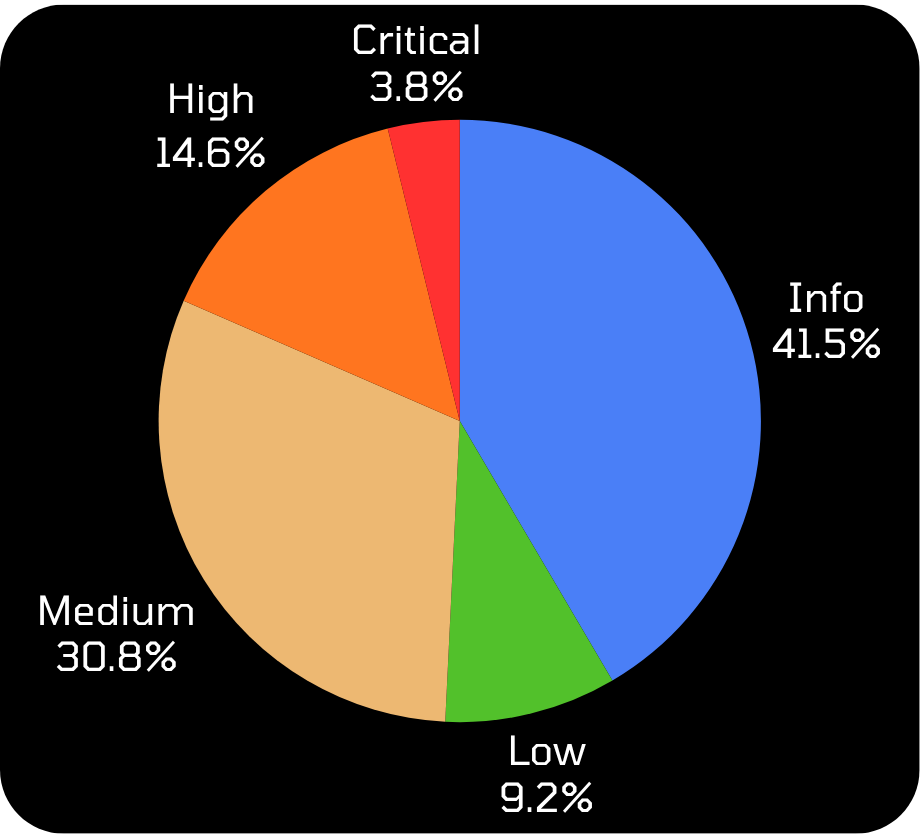
\includegraphics[width=0.7\textwidth]{assets/total-vulns.png}{Grafico a torta delle diverse vulnerabilità divise per livello}



















	\newpage
	\section{{DETAILED SUMMARY}}

	Le varie analisi condotte avvalendosi in modo combinato di strumenti quali \textbf{Nessus} (per le scansioni infrastrutturali e applicative web) e \textbf{OpenVAS}, hanno permesso un'\textbf{enumerazione precisa} delle varie vulnerabilità della macchina, identificandone il relativo \textbf{livello di pericolosità}. \\ 
	Il volume complessivo ha prodotto oltre \textbf{130 evidenze di sicurezza}. Al fine di restituire un quadro chiaro e privo di ridondanze, i risultati generati dai diversi scanner sono stati incrociati, filtrando i \textbf{falsi positivi}, escludendo le pure \textbf{note informative} (log/debug) e raggruppando i difetti per \textbf{tipologia di servizio esposto}. Di seguito si riporta l'inventario completo delle \textbf{criticità tecniche}, ordinate per \textbf{comparto logico}.
	\vspace{0.5cm}

	

	\subsection{{Catalogo Dettagliato delle Vulnerabilità}}

	\subsection*{\textbf{Classificazione del rischio}}
	Le analisi condotte avvalendosi in modo combinato di strumenti quali Nessus e OpenVAS hanno permesso un'enumerazione precisa delle varie vulnerabilità della macchina, identificandone il relativo livello di pericolosità. Il volume complessivo ha prodotto oltre 130 evidenze di sicurezza. Di seguito si riporta il dettaglio suddiviso per livello di criticità.

	\subsection{Vulnerabilità Critiche}

	\subsubsection{\textcolor{criticalred}{$\bullet$} RCE su servizio Samba trans2open -- CVE-2003-0201 (Analisi Manuale, OpenVAS, Nessus)}
	\fbox{\textbf{Descrizione:}} \\ \vspace{0.2 cm}
	Il sistema esegue Samba 2.2.1a, un servizio obsoleto esposto ad accessi non autenticati tramite Null Session. La vulnerabilità è causata da un Buffer Overflow nel demone \texttt{smbd} innescato durante l'elaborazione di messaggi SMB malformati di tipo \emph{Transaction2 Open}.

	\vspace{0.2 cm}
	\fbox{\noindent\textbf{Rischi:}} \\ \vspace{0.2 cm}
	L'attaccante può sfruttare il difetto di memoria per eseguire codice remoto arbitrario, ottenendo istantaneamente una shell con privilegi di root e il pieno controllo dell'asset.

	\vspace{0.2 cm}
	\fbox{\noindent\textbf{Contromisure:}} \\ \vspace{0.2 cm}
	Aggiornare il servizio Samba alla versione 2.2.8 o successiva, disabilitarlo se non strettamente necessario, oppure limitarne rigorosamente l'esposizione tramite firewall.

	\newpage
	\subsubsection{ \textcolor{criticalred}{$\bullet$} RCE su Apache mod\_ssl (OpenSSL-too-open) -- CVE-2002-0082 (Nessus, OpenVAS)}
	\fbox{\textbf{Descrizione:}} \\ \vspace{0.2 cm}
	Il server Apache utilizza il modulo \texttt{mod\_ssl} 2.8.4 vulnerabile. La debolezza, identificata tramite Nessus e OpenVAS, risiede in un Buffer Overflow che si manifesta durante la fase di handshake del protocollo SSLv2.

	\vspace{0.2 cm}
	\fbox{\noindent\textbf{Rischi:}} \\ \vspace{0.2 cm}
	Un attacco mirato consente la possibile esecuzione di codice arbitrario da remoto, permettendo all'attaccante di ottenere un primo accesso al server con i privilegi dell'utente \texttt{apache}.

	\vspace{0.2 cm}
	\fbox{\noindent\textbf{Contromisure:}} \\ \vspace{0.2 cm}
	Aggiornare la libreria OpenSSL a una release sicura e disabilitare completamente il supporto al protocollo crittografico obsoleto SSLv2.

	\subsubsection{ \textcolor{criticalred}{$\bullet$} Privilege Escalation tramite Kernel Linux (ptrace-kmod) -- CVE-2003-0127 (Analisi Manuale)}
	\fbox{\textbf{Descrizione:}} \\ \vspace{0.2 cm}
	Il sistema operativo si basa sul Kernel Linux 2.4, vulnerabile a causa di un grave difetto logico nella gestione combinata dei componenti \texttt{ptrace} e \texttt{kmod}. La falla è stata sfruttata localmente durante le attività di post-exploitation.

	\vspace{0.2 cm}
	\fbox{\noindent\textbf{Rischi:}} \\ \vspace{0.2 cm}
	Un attaccante che ha già ottenuto un accesso base al sistema può eseguire un'escalation immediata ai privilegi di root, aggirando le protezioni e compromettendo l'intera macchina.

	\vspace{0.2 cm}
	\fbox{\noindent\textbf{Contromisure:}} \\ \vspace{0.2 cm}
	Aggiornare radicalmente il sistema operativo e il kernel a distribuzioni e versioni moderne attivamente supportate.

	\newpage
	\subsection{Vulnerabilità Alte}

	\subsubsection{\textcolor{red}{$\bullet$} Deprecated SSH-1 Protocol Detection -- CVE-2001-0361, CVE-2001-0572 (Nessus, OpenVAS)}
	\fbox{\textbf{\textbf{Descrizione:}}}\\\vspace{0.2 cm}
	L'analisi del servizio esposto sulla porta 22/TCP ha rilevato il supporto attivo ai protocolli SSH-1, mantenuto a causa di una configurazione legacy non sicura.

	\vspace{0.2 cm}
	\fbox{\noindent\textbf{Rischi:}}\\\vspace{0.2 cm}
	L'utilizzo di un protocollo storicamente compromesso espone le sessioni di amministrazione remota a possibili intercettazioni e attacchi di tipo Man-in-the-Middle.

	\vspace{0.2 cm}
	\fbox{\textbf{\noindent\textbf{Contromisure:}}}\\\vspace{0.2 cm}
	Intervenire sul file di configurazione del demone SSH per forzare e consentire esclusivamente le connessioni tramite il protocollo moderno SSH-2.

	\subsubsection{\textcolor{red}{$\bullet$} Apache Chunked Encoding Remote Overflow -- CVE-2002-0392 (Nessus)}
	\fbox{\textbf{Descrizione:}} \\\vspace{0.2 cm}
	Vulnerabilità individuata tramite Nessus e localizzata nel parsing degli header HTTP da parte del server web Apache. Il difetto è generato da un Integer Overflow nella gestione dei trasferimenti con codifica chunked.

	\vspace{0.2 cm}
	\fbox{\noindent\textbf{Rischi:}} \\\vspace{0.2 cm}
	Lo sfruttamento intenzionale di questa debolezza può portare all'interruzione del servizio (DoS) o favorire l'esecuzione non autorizzata di codice remoto.

	\vspace{0.2 cm}
	\fbox{\noindent\textbf{Contromisure:}} \\\vspace{0.2 cm}
	Applicare tempestivamente le patch di sicurezza rilasciate per Apache o procedere all'aggiornamento dell'intero applicativo server.

	\subsection{Vulnerabilità Medie}

	\subsubsection{\textcolor{orange}{$\bullet$} Enumerazione Utenti tramite servizio Samba (Analisi Manuale)}
	\fbox{\textbf{Descrizione:}}\\	 \vspace{0.2 cm}	
	Durante le fasi di verifica manuale, è emerso che il servizio di condivisione Samba consente interrogazioni e accessi non autenticati utilizzando password nulle.

	\vspace{0.2 cm}
	\fbox{\noindent\textbf{Rischi:}}\\ \vspace{0.2 cm}
	 Un utente esterno malintenzionato può sfruttare questa apertura per estrarre informazioni sensibili, facilitando una rapida enumerazione degli utenti di sistema.

	\vspace{0.2 cm}
	\fbox{\noindent\textbf{Contromisure:}} \\ \vspace{0.2 cm}
	Riconfigurare i permessi del servizio Samba, bloccando in modo categorico la possibilità di stabilire Null Session anonime.


	\subsubsection{\textcolor{orange}{$\bullet$} HTTP TRACE / TRACK Methods Allowed -- CVE-2003-1567 (Nessus)}
	\fbox{\textbf{Descrizione:}} \\ \vspace{0.2 cm}
	La verifica dei metodi HTTP supportati ha evidenziato che i comandi di debugging TRACE e TRACK sono attivi, indicando un marcato mancato hardening del server web.

	\vspace{0.2 cm}
	\fbox{\noindent\textbf{Rischi:}}\\ \vspace{0.2 cm}
	L'attivazione di questi metodi diagnostici facilita la conduzione di possibili attacchi Cross-Site Tracing (XST) contro gli utenti che navigano l'applicativo.

	\vspace{0.2 cm}
	\fbox{\noindent\textbf{Contromisure:}}\\ \vspace{0.2 cm}
	Disabilitare esplicitamente il metodo configurando la direttiva \texttt{TraceEnable Off} all'interno del file di configurazione di Apache.


	\subsubsection{\textcolor{orange}{$\bullet$} Webalizer Cross Site Scripting -- CVE-2001-0835 (Nessus, OpenVAS)}
	\fbox{\textbf{Descrizione:}} \\ \vspace{0.2 cm}
	L'analisi delle directory web esposte ha portato alla luce una vulnerabilità XSS presente nell'applicativo Webalizer. Il problema deriva da una sanitizzazione insufficiente degli input processati.

	\vspace{0.2 cm}
	\fbox{\noindent\textbf{Rischi:}} \\ \vspace{0.2 cm}
	Un attaccante potrebbe indurre il browser di una vittima a eseguire script malevoli, causando il furto di sessione o l'esecuzione di azioni arbitrarie non autorizzate.

	\vspace{0.2 cm}
	\fbox{\noindent\textbf{Contromisure:}} \\ \vspace{0.2 cm}
	Aggiornare il software Webalizer a una versione sicura o, qualora non strettamente necessario, rimuoverne l'installazione dal server web.

	\subsection{Vulnerabilità Basse}

	\subsubsection{\textcolor{green}{$\bullet$} ICMP Timestamp Reply Information Disclosure -- CVE-1999-0524 (Nessus, OpenVAS)}
	\fbox{\textbf{Descrizione:}} \\\vspace{0.2 cm}
	Inviando specifiche richieste ICMP di Type 13, è stato confermato che il sistema target restituisce risposte ai pacchetti ICMP Timestamp.

	\vspace{0.2 cm}
	\fbox{\noindent\textbf{Rischi:}} \\\vspace{0.2 cm}
	Questo comportamento agevola la raccolta di informazioni temporali e operative sul sistema, facilitando la fase di ricognizione.









	\newpage
	\section{Considerazioni finali}

	L'attività di \textbf{Penetration Testing} condotta sull'infrastruttura \textbf{Kioptrix Level 1} ha fatto emergere un quadro di sicurezza estremamente critico. La presenza di vulnerabilità storiche, ampiamente documentate e di pubblico dominio, combinata con l'assenza di una politica di aggiornamento strutturale, espone l'asset a compromissioni totali e immediate da parte di attaccanti esterni, operanti anche in totale assenza di credenziali valide.\\
	Il conseguimento dei massimi privilegi di sistema (\textbf{root}) attraverso molteplici e distinti vettori di attacco (servizio Samba, modulo OpenSSL e Kernel Linux) dimostra in modo inequivocabile che l'attuale configurazione non è in grado di garantire i requisiti minimi di \textbf{Riservatezza, Integrità e Disponibilità} dei dati aziendali.\\
	Si raccomanda ai referenti dell'infrastruttura di procedere con \textbf{estrema urgenza} all'applicazione del piano di mitigazione illustrato nel presente report. Nello specifico, data l'obsolescenza profonda delle componenti (come il Kernel obsoleto), si sconsiglia il semplice "patching" dei singoli servizi in favore di una \textbf{migrazione completa del sistema operativo} verso distribuzioni moderne, attivamente supportate e dotate di difese in memoria native.\\
	Fino al completamento e alla validazione di tali interventi di sicurezza, l'asset deve essere considerato \textbf{altamente vulnerabile} e deve essere, se possibile, \textbf{isolato a livello perimetrale} come un utilizzo di Firewall per prevenire incidenti di sicurezza che potrebbero potenzialmente estendersi in un'ipotetica rete esterna.

	\newpage
	\section{Riferimenti bibliografici}

	\begin{thebibliography}{99}

	\bibitem{cve-2003-0201}
	National Vulnerability Database (NVD) -- NIST.\\
	\textbf{CVE-2003-0201} -- Samba \textit{call\_trans2open} Remote Buffer Overflow.\\
	Buffer overflow nella funzione \texttt{call\_trans2open} di \texttt{trans2.c} in Samba 2.2.x
	(prima della 2.2.8a), che consente a un attaccante remoto di eseguire codice arbitrario.\\
	\url{https://nvd.nist.gov/vuln/detail/CVE-2003-0201}



	\bibitem{cve-2002-0082}
	National Vulnerability Database (NVD) -- NIST.\\
	\textbf{CVE-2002-0082} -- Apache \texttt{mod\_ssl} $<$ 2.8.7 (\textit{OpenSSL-too-open}) Remote Buffer Overflow.\\
	Il codice di gestione delle sessioni (dbm e shm) in \texttt{mod\_ssl} prima della versione 2.8.7-1.3.23
	non inizializza correttamente la memoria tramite la funzione \texttt{i2d\_SSL\_SESSION},
	permettendo a un attaccante remoto di eseguire codice arbitrario tramite un Buffer Overflow.\\
	\url{https://nvd.nist.gov/vuln/detail/CVE-2002-0082}



	\bibitem{cve-2003-0127}
	National Vulnerability Database (NVD) -- NIST.\\
	\textbf{CVE-2003-0127} -- Linux Kernel \textit{ptrace/kmod} Local Privilege Escalation.\\
	Il loader dei moduli del kernel Linux 2.2.x (prima della 2.2.25) e 2.4.x (prima della 2.4.21)
	consente agli utenti locali di ottenere privilegi di root sfruttando \texttt{ptrace} per agganciarsi
	a un processo figlio avviato dal kernel.\\

	\url{https://nvd.nist.gov/vuln/detail/CVE-2003-0127}

	\bibitem{poodle}
	National Vulnerability Database (NVD) -- NIST.\\
	\textbf{CVE-2014-3566} -- POODLE: Padding Oracle On Downgraded Legacy Encryption (SSLv3).\\
	\url{https://nvd.nist.gov/vuln/detail/CVE-2014-3566}



	\bibitem{sweet32}
	National Vulnerability Database (NVD) -- NIST.\\
	\textbf{CVE-2016-2183} -- SWEET32: Birthday Attack su cifrari a blocchi a 64-bit (3DES, Blowfish).\\
	\url{https://nvd.nist.gov/vuln/detail/CVE-2016-2183}



	\bibitem{freak}
	National Vulnerability Database (NVD) -- NIST.\\
	\textbf{CVE-2015-0204} -- FREAK: RSA Export Keys Downgrade Attack.\\
	\url{https://nvd.nist.gov/vuln/detail/CVE-2015-0204}

	\bibitem{logjam}
	National Vulnerability Database (NVD) -- NIST.\\
	\textbf{CVE-2015-4000} -- Logjam: Attacco di downgrade su DHE\_EXPORT (Diffie-Hellman a 512-bit).\\
	\url{https://nvd.nist.gov/vuln/detail/CVE-2015-4000}

	\bibitem{drown}
	National Vulnerability Database (NVD) -- NIST.\\
	\textbf{CVE-2016-0800} -- DROWN: Decrypting RSA with Obsolete and Weakened eNcryption (SSLv2 cross-protocol attack).\\
	\url{https://nvd.nist.gov/vuln/detail/CVE-2016-0800}

	\bibitem{metasploit}
	Rapid7.\\
	\textbf{Metasploit Framework} -- Framework open-source per lo sviluppo e l'esecuzione di exploit.\\
	Utilizzato nel test per sfruttare le vulnerabilità \textit{trans2open} (CVE-2003-0201).\\
	\url{https://www.metasploit.com}

	\bibitem{nessus}
	Tenable, Inc.\\
	\textbf{Nessus} -- Scanner di vulnerabilità di rete. Versione utilizzata: Basic Network Scan \& Web Application Tests.\\
	\url{https://www.tenable.com/products/nessus}

	\bibitem{openvas}
	Greenbone Networks.\\
	\textbf{OpenVAS (Open Vulnerability Assessment System)} -- Scanner di vulnerabilità open-source.
	Versione utilizzata: configurazione \textit{Full and Fast}.\\
	\url{https://www.greenbone.net/en/vulnerability-management/}

	\bibitem{nikto}
	CIRT.net.\\
	\textbf{Nikto} -- Web server scanner open-source per l'identificazione di vulnerabilità nei server HTTP/HTTPS.\\
	\url{https://cirt.net/Nikto2}

	\bibitem{dirb}
	The Security Factory.\\
	\textbf{DIRB} -- Web content scanner per l'enumerazione di directory e file nascosti su server web.\\
	\url{https://dirb.sourceforge.net}

	\bibitem{gobuster}
	OJ Reeves.\\
	\textbf{Gobuster} -- Tool di directory/file brute-forcing scritto in Go, utilizzato per il crawling del server Apache.\\
	\url{https://github.com/OJ/gobuster}

	\bibitem{rpcclient}
	Samba Team.\\
	\textbf{rpcclient} -- Utility del pacchetto Samba per l'interrogazione di servizi RPC/SMB remoti.
	Utilizzata per verificare l'accesso non autenticato (Null Session) al servizio Samba.\\
	\url{https://www.samba.org/samba/docs/current/man-html/rpcclient.1.html}

	\bibitem{cvss}
	FIRST (Forum of Incident Response and Security Teams).\\
	\textbf{Common Vulnerability Scoring System (CVSS) v3.1} -- Standard per la valutazione della severità delle vulnerabilità.\\
	\url{https://www.first.org/cvss/specification-document}

	\bibitem{nvd}
	National Institute of Standards and Technology (NIST).\\
	\textbf{National Vulnerability Database (NVD)} -- Database ufficiale delle vulnerabilità note.\\
	\url{https://nvd.nist.gov}
	\end{thebibliography}



\end{document}





	\begin{comment}
	\begin{abstract}
		Il documento è un \textbf{Penetration Testing Report} relativo alla macchina "Kioptrix Level 1". 
		Ci si è occupati nel scrivere nel dettaglio le varie sezioni quali: executive summary , engagement highlights, vulnerability report, remediation report, findings summary e detailed summary. 
		
		L'attività del penetration testing ha simulato un attacco informatico di tipo "\textbf{BlackBox}" per identificare le vulnerabilità del sistema, rilevando 130 evidenze di insicurezza dell' oerativo di test, di cui 3 di livello critico (CVSS 10.0). 
		
		Il presente documento illustra i vettori di attacco, l'impatto sulla sicurezza e fornisce un piano dettagliato di mitigazione per la risoluzione delle falle.
	\end{abstract}
	\end{comment}
